%%%%%%%%%%%%%%%%%%%%%%%%%%%%%%%%%%%%%%%%%
% Beamer Presentation
% LaTeX Template
% Version 1.0 (10/11/12)
%
% This template has been downloaded from:
% http://www.LaTeXTemplates.com
%
% License:
% CC BY-NC-SA 3.0 (http://creativecommons.org/licenses/by-nc-sa/3.0/)
%
%%%%%%%%%%%%%%%%%%%%%%%%%%%%%%%%%%%%%%%%%

%----------------------------------------------------------------------------------------
%	PACKAGES AND THEMES
%----------------------------------------------------------------------------------------

\documentclass{beamer}

\mode<presentation> {

% The Beamer class comes with a number of default slide themes
% which change the colors and layouts of slides. Below this is a list
% of all the themes, uncomment each in turn to see what they look like.

%\usetheme{default}
%\usetheme{AnnArbor}
%\usetheme{Antibes}
%\usetheme{Bergen}
%\usetheme{Berkeley}
%\usetheme{Berlin}
%\usetheme{Boadilla}
%\usetheme{CambridgeUS}
%\usetheme{Copenhagen}
%\usetheme{Darmstadt}
%\usetheme{Dresden}
%\usetheme{Frankfurt}
%\usetheme{Goettingen}
%\usetheme{Hannover}
%\usetheme{Ilmenau}
%\usetheme{JuanLesPins}
%\usetheme{Luebeck}
\usetheme{uu}
%\usetheme{Malmoe}
%\usetheme{Marburg}
%\usetheme{Montpellier}
%\usetheme{PaloAlto}
%\usetheme{Pittsburgh}
%\usetheme{Rochester}
%\usetheme{Singapore}
%\usetheme{Szeged}
%\usetheme{Warsaw}

% As well as themes, the Beamer class has a number of color themes
% for any slide theme. Uncomment each of these in turn to see how it
% changes the colors of your current slide theme.

%\usecolortheme{albatross}
%\usecolortheme{beaver}
%\usecolortheme{beetle}
%\usecolortheme{crane}
%\usecolortheme{dolphin}
%\usecolortheme{dove}
%\usecolortheme{fly}
%\usecolortheme{lily}
\usecolortheme{orchid}
%\usecolortheme{rose}
%\usecolortheme{seagull}
%\usecolortheme{seahorse}
%\usecolortheme{whale}
%\usecolortheme{wolverine}

%\setbeamertemplate{footline} % To remove the footer line in all slides uncomment this line
%\setbeamertemplate{footline}[page number] % To replace the footer line in all slides with a simple slide count uncomment this line

%\setbeamertemplate{navigation symbols}{} % To remove the navigation symbols from the bottom of all slides uncomment this line
}

\usepackage{graphicx} % Allows including images
\usepackage{booktabs} % Allows the use of \toprule, \midrule and \bottomrule in tables
\usepackage[english]{babel}
\usepackage{graphics}
\usepackage{color}
\usepackage[latin1]{inputenc}
\usepackage{tikz}
\def\checkmark{\tikz\fill[scale=0.4](0,.35) -- (.25,0) -- (1,.7) -- (.25,.15) -- cycle;} 
\usepackage{times}
\usepackage[T1]{fontenc}
%----------------------------------------------------------------------------------------
%	TITLE PAGE
%----------------------------------------------------------------------------------------
\setlength\fboxsep{0pt}
\setlength\fboxrule{0.5pt}

\title[Extending Bayesian analysis of circular data]{Extending Bayesian analysis of circular data for comparison of multiple groups} % The short title appears at the bottom of every slide, the full title is only on the title page

\author{Kees Mulder} % Your name
\institute[UU] % Your institution as it will appear on the bottom of every slide, may be shorthand to save space
{
Utrecht University \\ % Your institution for the title page
\medskip
\textit{k.t.mulder@uu.nl} % Your email address
}
\date{September 19, 2014} % Date, can be changed to a custom date

\begin{document}

\begin{frame}
\titlepage
\end{frame}

\section{What is circular data?}

\begin{frame}

\begin{center}
\pause
\vspace{1.7cm}
\begin{minipage}{\framewidth}
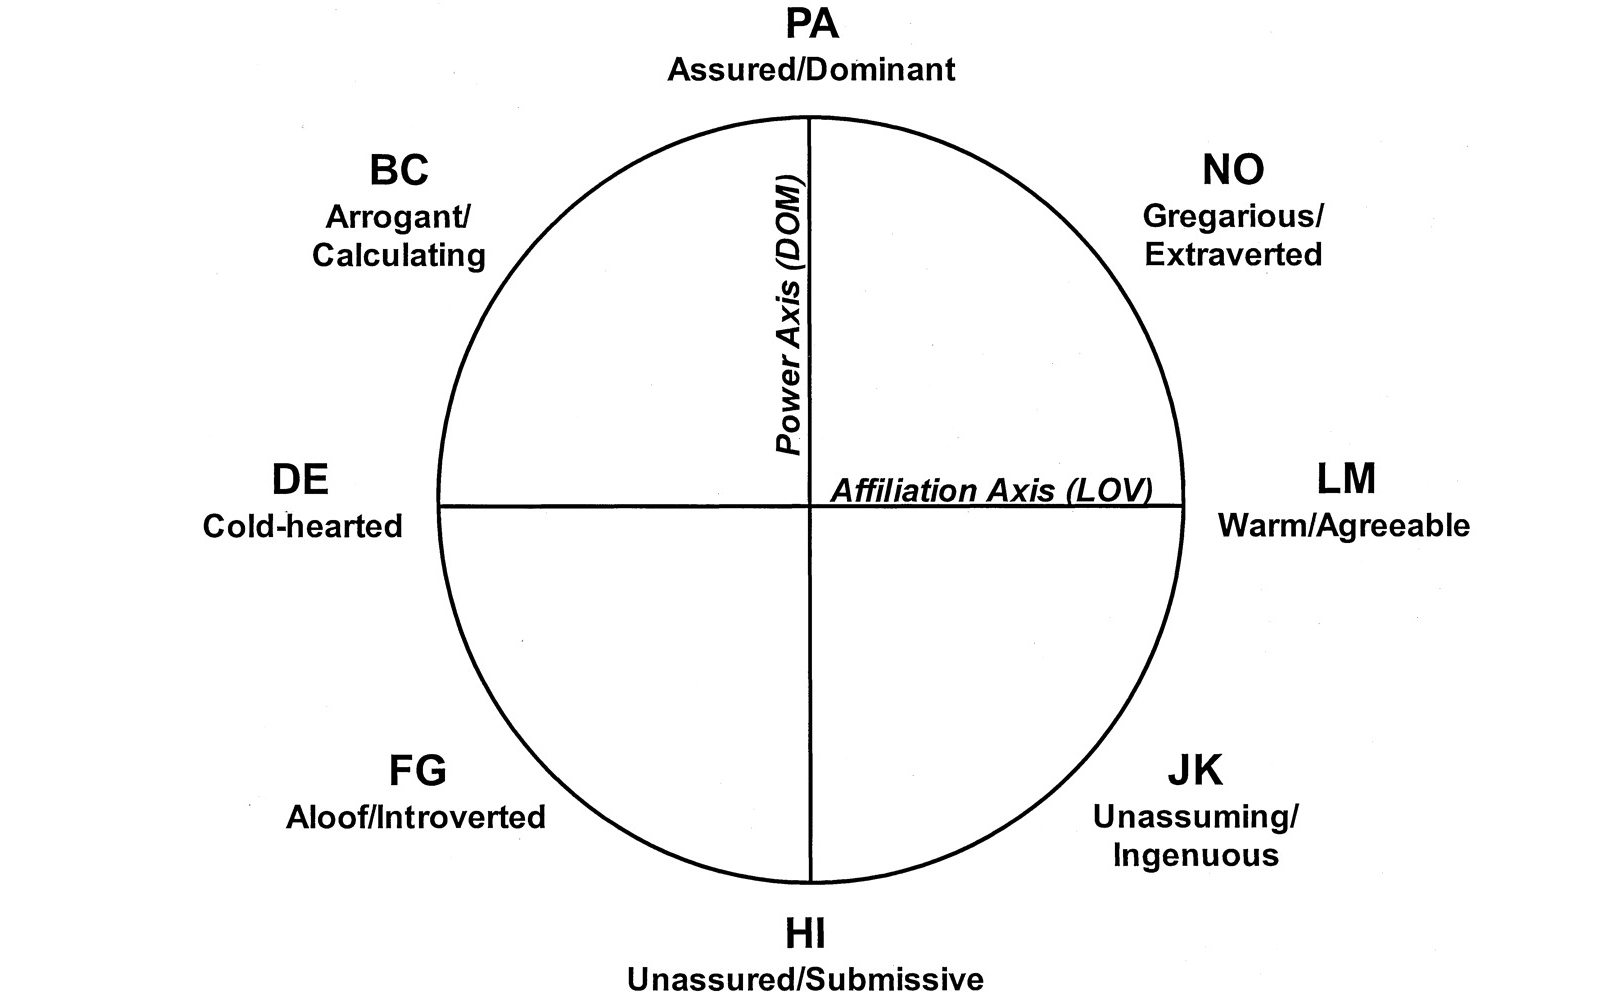
\includegraphics[width=0.88\textwidth]{Examplepics/Leary.jpg}
\vspace{0.6cm}
\end{minipage}
\begin{minipage}{\framewidth}

\begin{center}
\begin{tabular}{lcccc}
         & \multicolumn{4}{c}{ } \\
 &&&& \\
 &&&& \\
\end{tabular}
\end{center}
\vspace{0.6cm}
\end{minipage}
%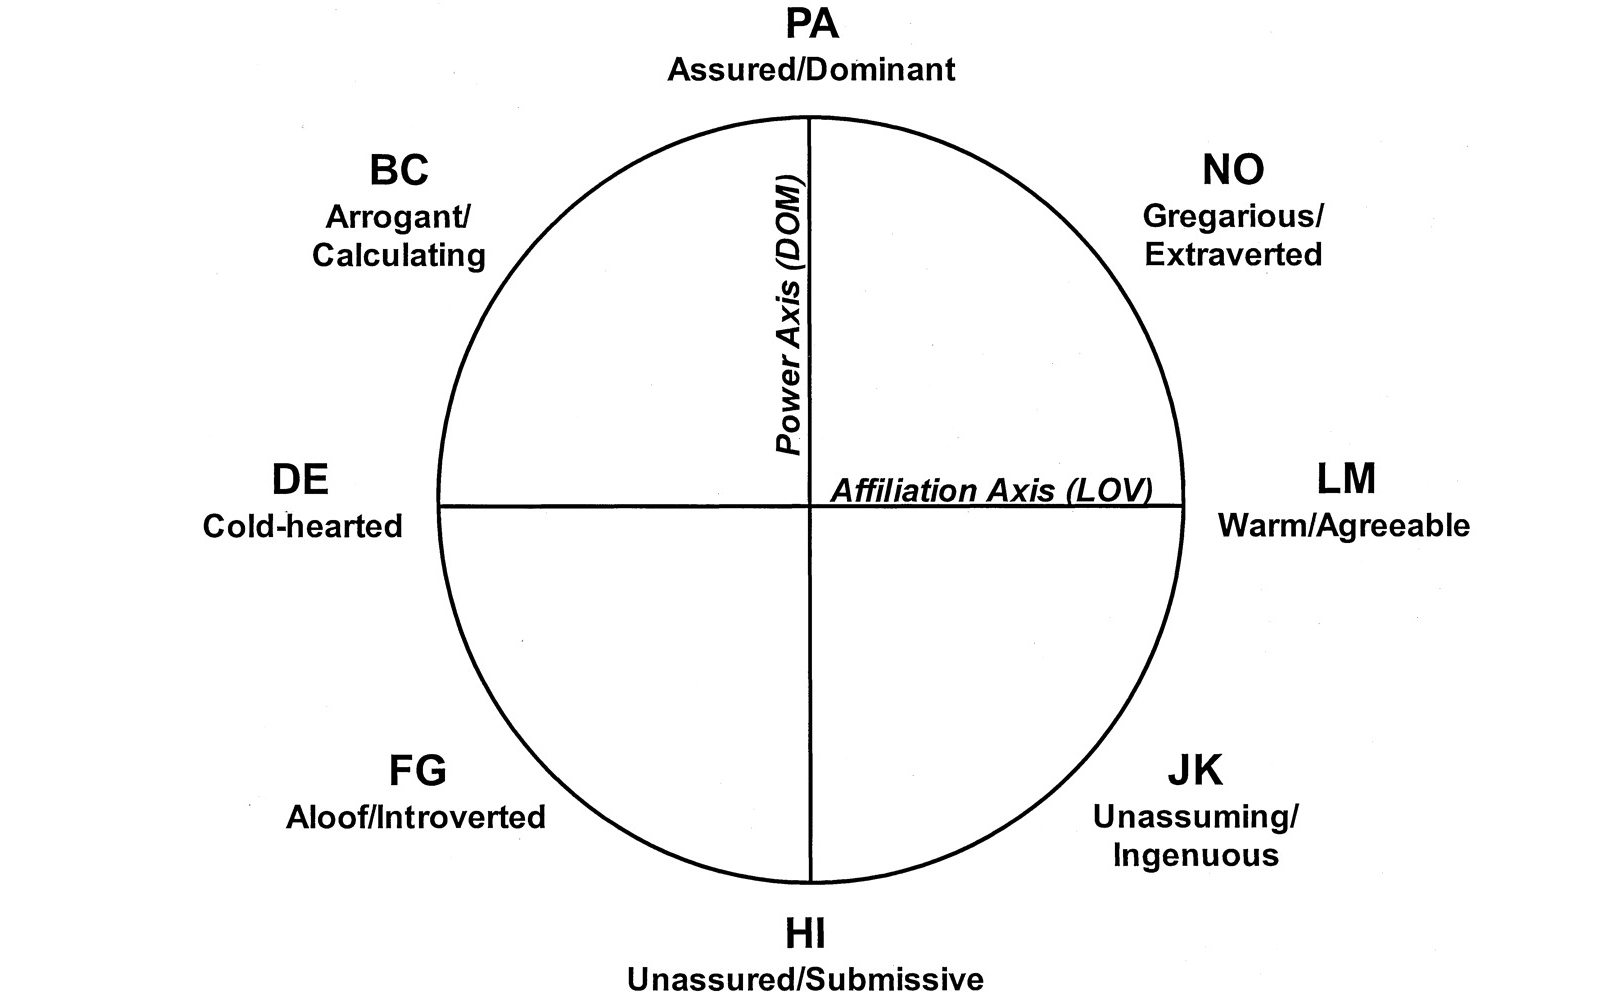
\includegraphics[width=0.88\textwidth]{Examplepics/Leary.jpg}
\end{center}
\end{frame}



\begin{frame}
\begin{center}
\begin{minipage}{\framewidth}
\begin{center}
\begin{tabular}{lcccc}
         & \multicolumn{4}{c}{Score on Leary's rose} \\ \cmidrule{1-5}
Managers & $46^\circ$ & $92^\circ$ & $102^\circ$ & $122^\circ$ \\
Teachers & $80^\circ$ & $47^\circ$ & $5^\circ$ & $355^\circ$ \\
\end{tabular}
\end{center}
\end{minipage}
\begin{minipage}[l]{0.42\framewidth}
\uncover<2->{\fbox{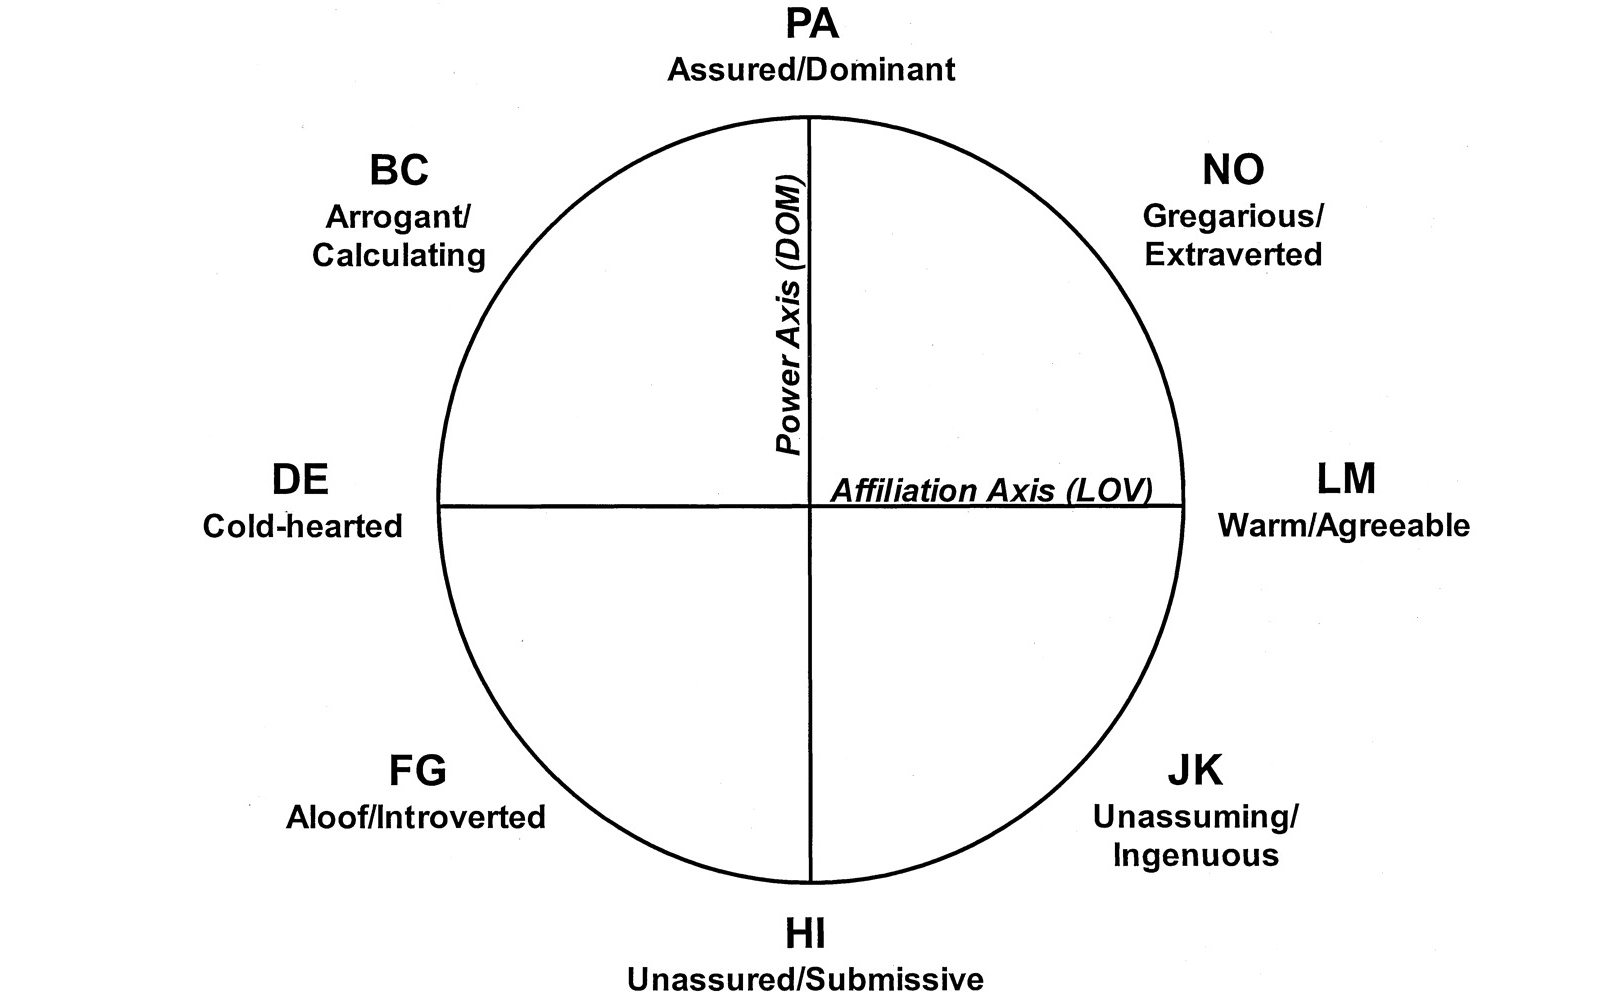
\includegraphics[width=\textwidth]{Examplepics/Leary.jpg}}}\vspace{0.1cm}
\uncover<4->{\fbox{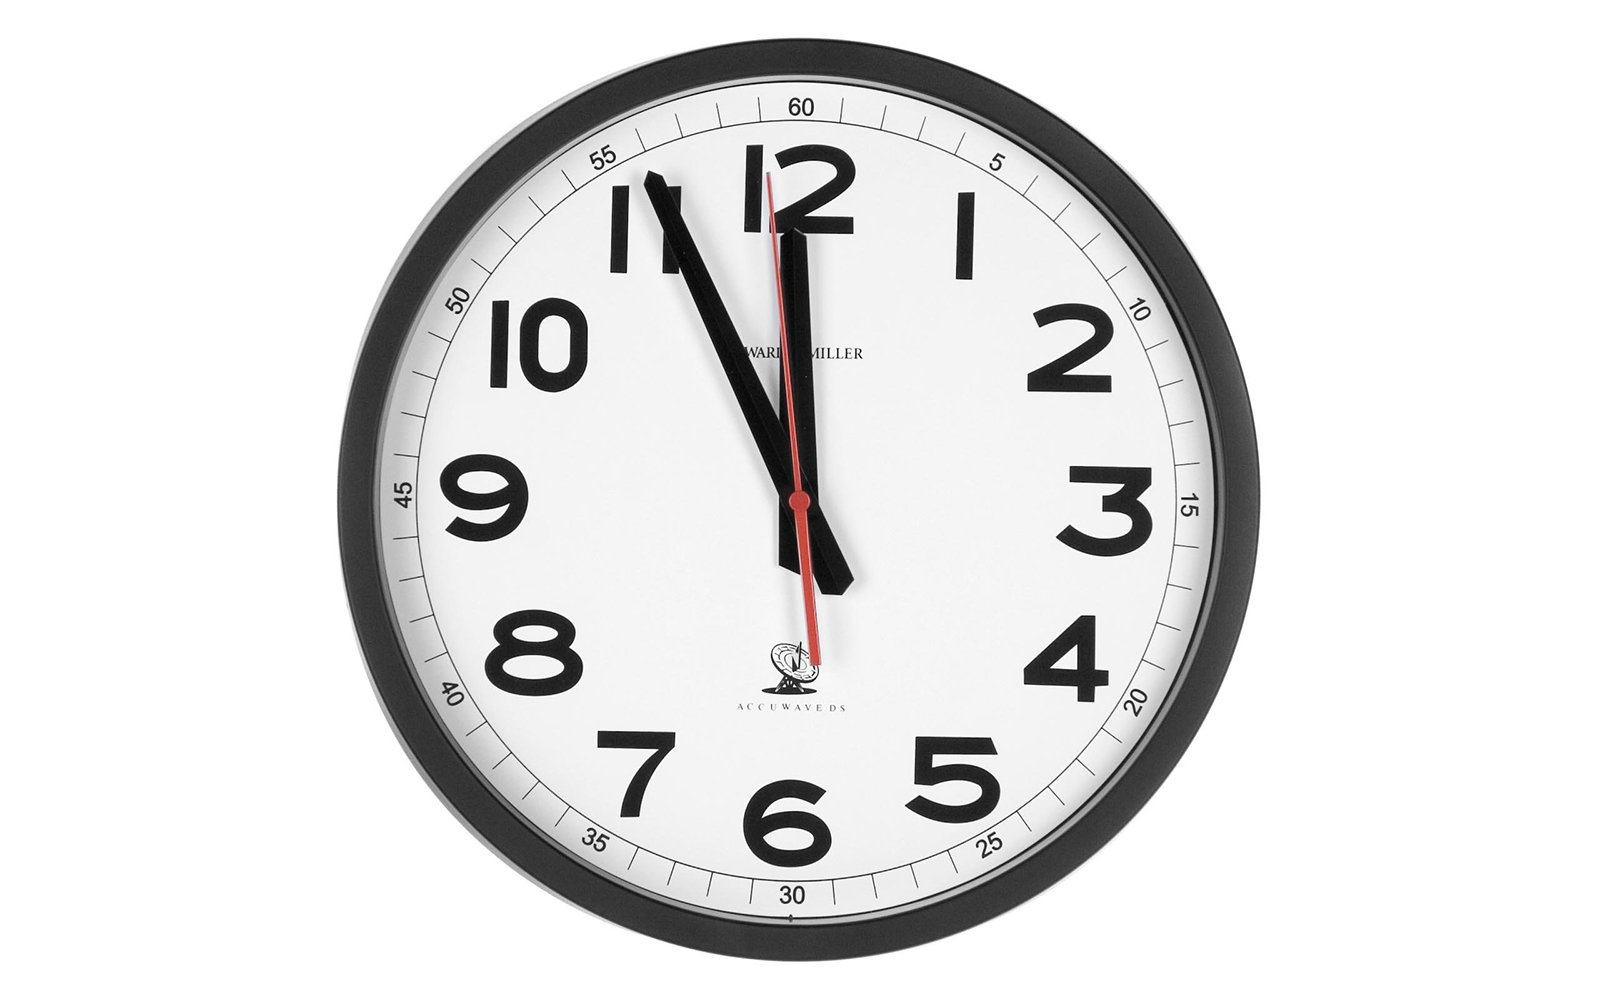
\includegraphics[width=\textwidth]{Examplepics/Clock.jpg}}}
\end{minipage}
\begin{minipage}[r]{0.42\framewidth}
\uncover<3->{\fbox{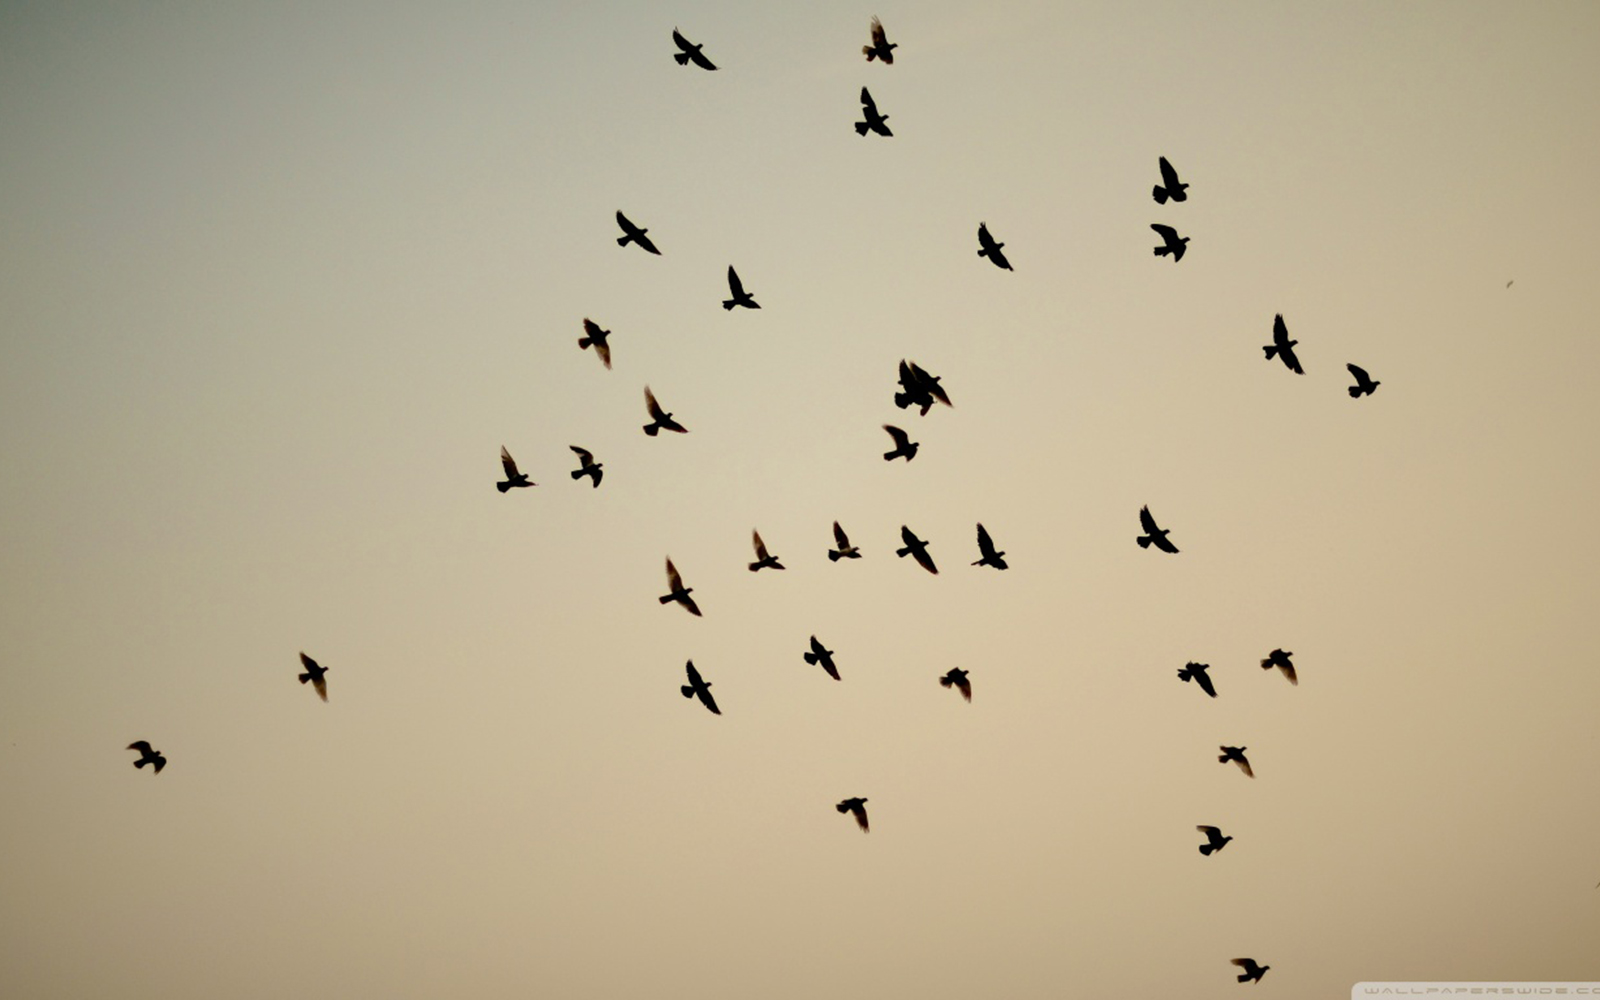
\includegraphics[width=\textwidth]{Examplepics/Birds.jpg}}}\vspace{0.1cm}
\uncover<5->{\fbox{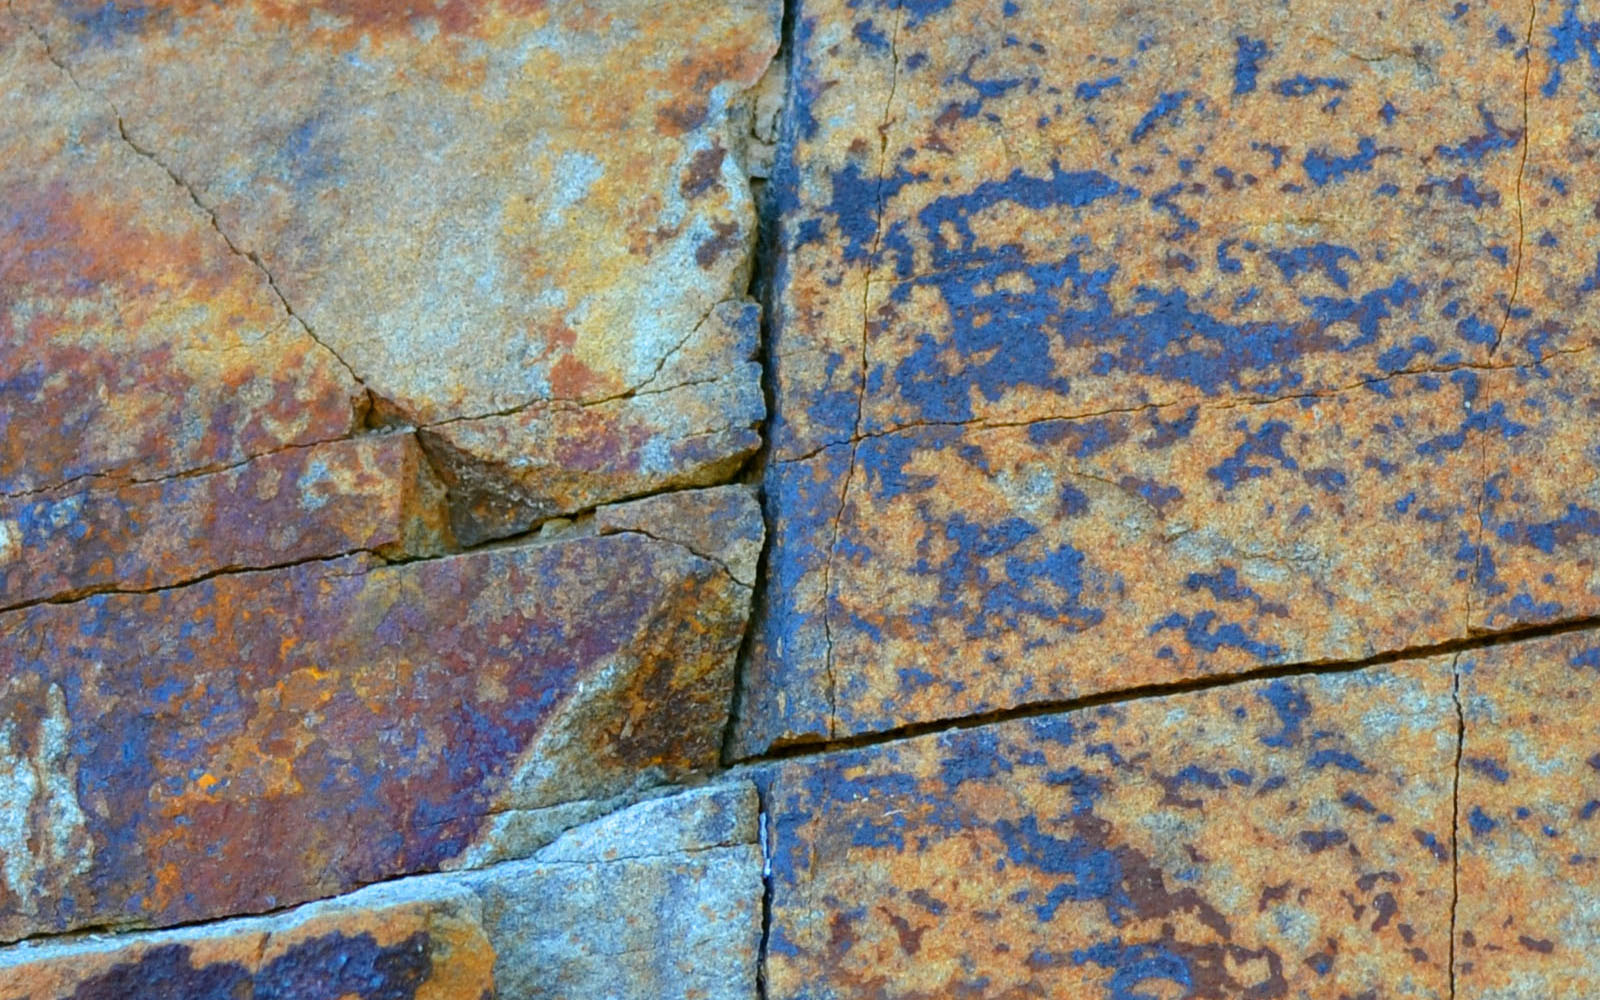
\includegraphics[width=\textwidth]{Examplepics/Rocks.jpg}}}
\end{minipage}
\end{center}
\end{frame}






\section{Can we analyze it?}

\subsection{Difference with linear}

\begin{frame}
\begin{center}

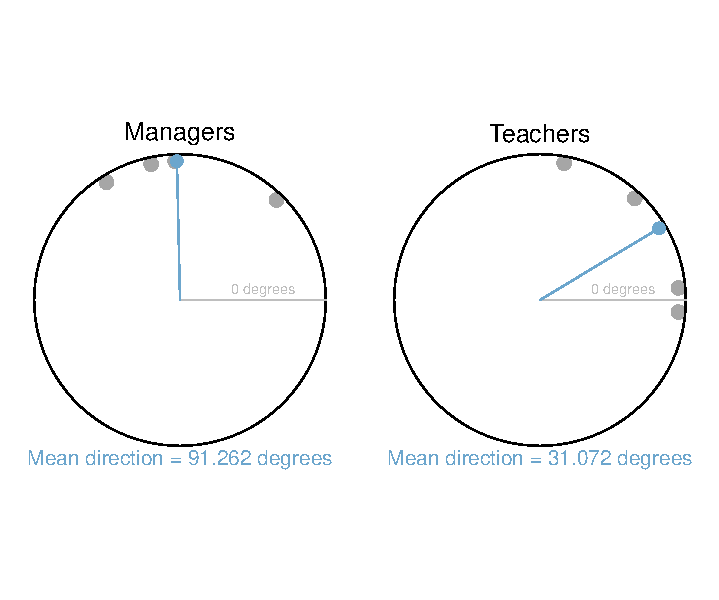
\includegraphics[width=0.7\textwidth, clip=true, trim=0.4cm 2cm 0.4cm 2cm]{ManagersTeachers.pdf}
\vspace{0.5cm}

\pause

\textbf{Difference with linear data} \pause
\begin{itemize}
	\item Teacher with score 5$^\circ$ \pause
	\item Teacher with score 355$^\circ$ \pause
	\item Linear methods: difference of 350$^\circ$ \pause
	\item Difference is really only 10$^\circ$ \pause
	\item \textbf{Linear methods can not be used}
\end{itemize}

\end{center}
\end{frame}



\begin{frame}
\begin{center}

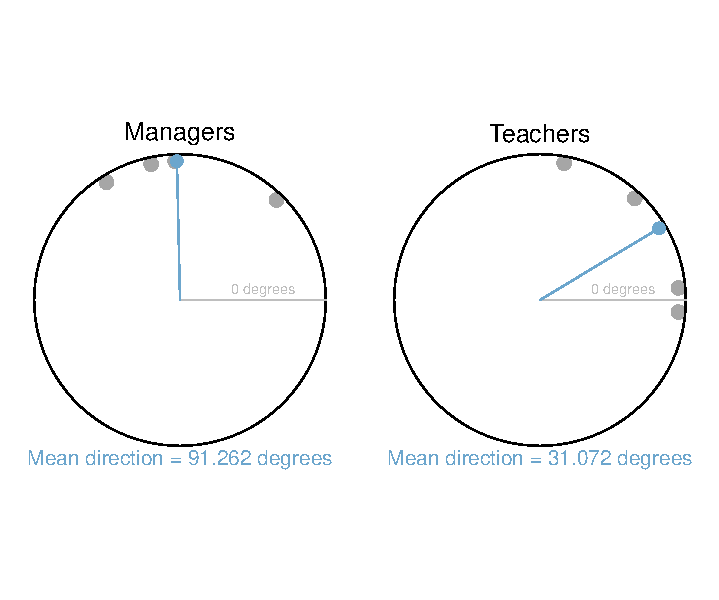
\includegraphics[width=0.7\textwidth, clip=true, trim=0.4cm 2cm 0.4cm 2cm]{ManagersTeachers.pdf}
\vspace{0.5cm}

%\textbf{Circular data}
\begin{itemize}
\item Inherently difficult to analyse
\pause
\item Bayesian methods may prove useful $\rightarrow$ flexible
\pause
\item Three approaches are used
\end{itemize}

\end{center}
\end{frame}

\subsection{Three available methods}



\begin{frame}{Intrinsic Approach}

\begin{itemize}

\item Define distributions on the circle
\pause
\item Sample space: $\mathbb{S}^1$
\pause

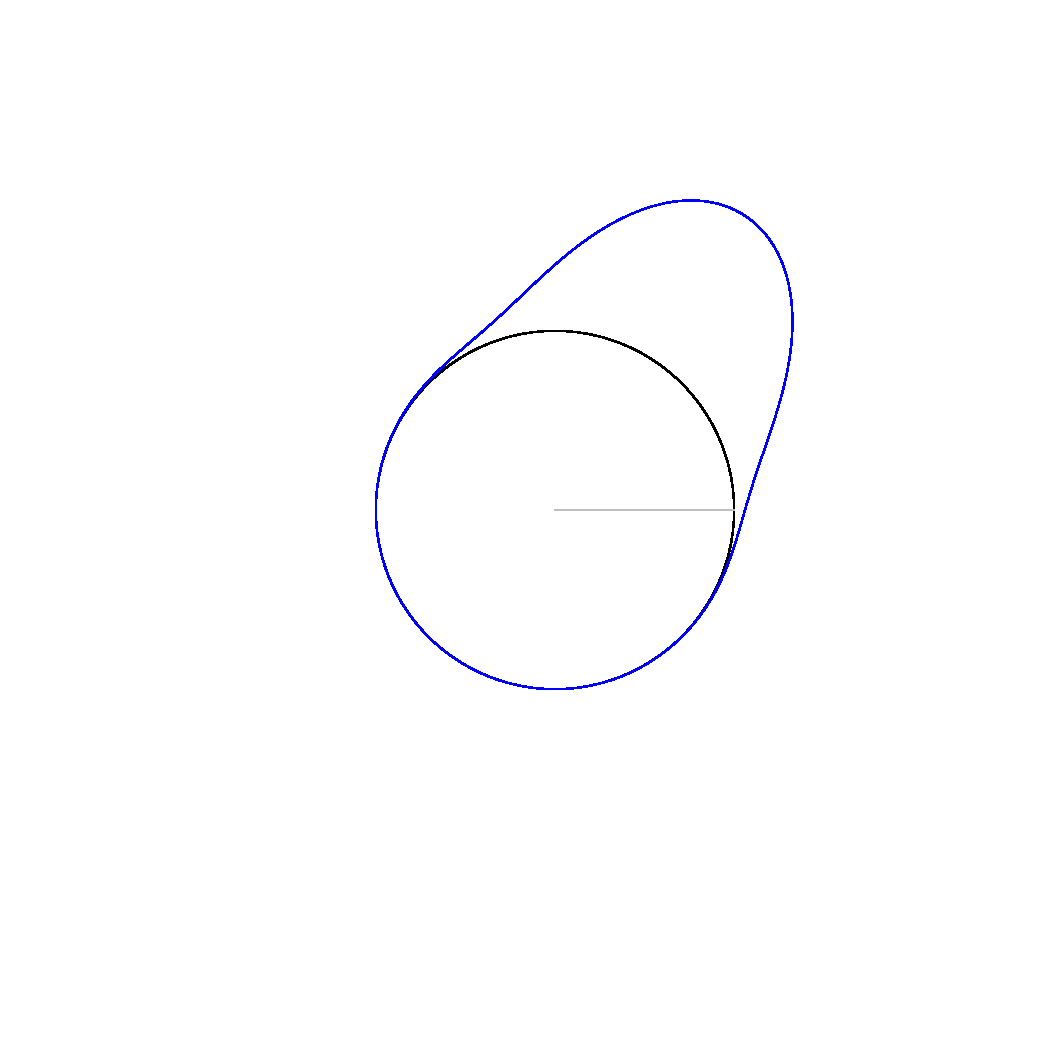
\includegraphics[width=0.5\textwidth, clip=true, trim = 3cm 6cm 3cm 3.3cm]{vonMises.pdf}

\pause

\item Example: von Mises distribution \pause
$$ \textnormal{VM}(\theta \vert \mu, \kappa) = \frac{  \exp\{\kappa \cos(\theta - \mu)\} }{2 \pi I_0(\kappa) } , 0\leq \theta < 2\pi, \kappa \geq 0$$

\end{itemize}



\begin{description}
\pause
\item[Pro] Straightforward
\pause
\item[Con] Bessel function 

\end{description}

\end{frame}




\begin{frame}{Wrapped Approach}

\begin{itemize}

\item<1-> 'Wrap' distribution on the real line to the circle
\item<1-> Map: $\mathbb{S}^1 \to \mathbb{R}^1$

\includegraphics<1>[width=0.5\textwidth]{UnwrapOnCircle.pdf}
\includegraphics<2>[width=0.5\textwidth]{UnwrapData.pdf}
\includegraphics<3>[width=0.5\textwidth]{UnwrapMoved.pdf}
\includegraphics<4->[width=0.5\textwidth]{UnwrapDensity.pdf}

\end{itemize}

\vspace{-0.8cm}

\begin{description}
%\pause 
\item<5->[Pro] May use linear methods
%\pause
\item<6->[Con] Wrapping process

\end{description}

\end{frame}





\begin{frame}{Embedding Approach}

\begin{itemize}

\item<1-> 'Project' distribution in two-dimensional space to the circle
\item<1-> Map: $\mathbb{S}^1 \to \mathbb{R}^2$
 
\includegraphics<1>[width=0.5\textwidth]{ProjectOnCircle.pdf}
\includegraphics<2>[width=0.5\textwidth]{ProjectContourOnly.pdf}
\includegraphics<3>[width=0.5\textwidth]{ProjectPoints.pdf}
\includegraphics<4->[width=0.5\textwidth]{ProjectDensity.pdf}

\end{itemize}

\vspace{-0.8cm}

\begin{description}
%\pause 
\item<5->[Pro] May use bivariate linear methods
%\pause
\item<6->[Con] Complex, heteroscedasticity
 
\end{description}

\end{frame}


\begin{frame}
Which approach?
\begin{itemize}
\item Wrapping, embedding: practical solutions
\item Intrinsic: most natural, direct
\end{itemize}

\end{frame}




\subsection{What's missing?}


\begin{frame}
\begin{center}

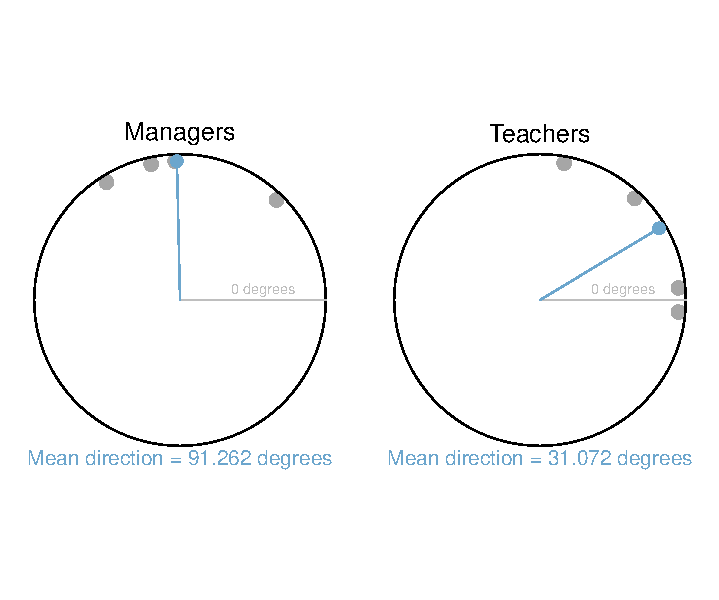
\includegraphics[width=0.7\textwidth, clip=true, trim=0.4cm 2cm 0.4cm 2cm]{ManagersTeachers.pdf}
\vspace{0.5cm}

\textbf{Intrinsic approach: what's missing?}
\begin{itemize}
\item Methods analyze a single group of data
\pause
\item We need \textbf{multiple groups} \pause with \textbf{common variance}

\end{itemize}

\end{center}
\end{frame}



\section{Contributions}


\begin{frame}
\frametitle{Previous methods}

\def\arraystretch{1.5}
\begin{table}
\begin{tabular}{lcc}
\textbf{Method} & \textbf{Prior} & \textbf{Multiple groups} \\\hline
Gibbs sampler & \checkmark & $\times$ \\
%Metropolis-Hastings  & $\times$ & $\times$ \\
Rejection sampler & $\times$ & $\times$ \\
  &  &  \\
\end{tabular}
%\caption{Previously available of MCMC-methods for analysis of von Mises circular data}
\end{table}
\end{frame}

\begin{frame}
\frametitle{Extensions}

\def\arraystretch{1.5}
\begin{table}
\begin{tabular}{lcc}
\textbf{Method} & \textbf{Prior} & \textbf{Multiple groups} \\\hline
Gibbs sampler & \checkmark & \checkmark \\
Rejection sampler & \checkmark & \checkmark \\

 \color{blue} Metropolis-Hastings  & \color{blue} \checkmark & \color{blue} \checkmark \\ 

\end{tabular}
%\caption{Current status of MCMC-methods for analysis of von Mises circular data}
\end{table}
\end{frame}



\subsection{von Mises distribution}

\begin{frame}{Circular summary statistics}

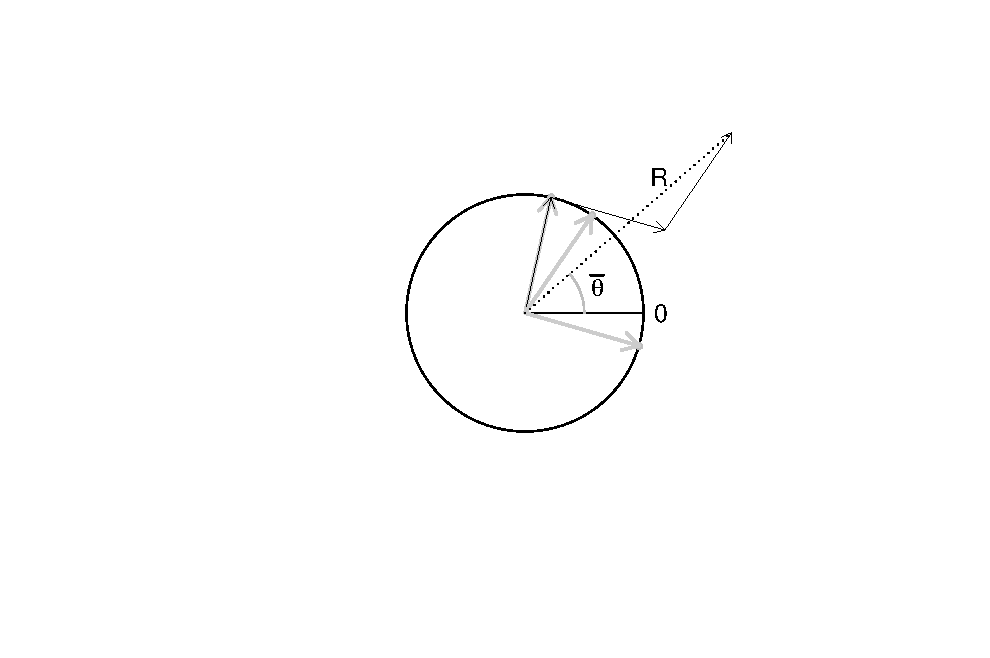
\includegraphics[width=1\linewidth, clip, trim= 4cm 3cm 1cm 2cm]{/home/kees/Dropbox/Masterthesis/Writing/Kees/Thesis/ExampleRMu}

\begin{itemize}
\item $\bar\theta$: Unbiased estimate of $\mu$
\item R: Resultant length
\end{itemize}

\end{frame}


\begin{frame}{von Mises posterior}	

We can use a conjugate prior:

$$ p(\mu, \kappa) \propto \frac{\exp\{R_0 \kappa \cos (\mu - \mu_0)\}  } {I_0 (\kappa) ^{c}} ,$$

The posterior for multiple groups with a common $\kappa$ is given by $$f(\boldsymbol{\mu}, \kappa \vert \boldsymbol\theta) \propto \{I_0 (\kappa) \}^{-m_t} \exp \left[ \kappa \sum_{j=1}^{J} R_{nj} \cos (\mu_j - \mu_{nj})\right], $$ where $\boldsymbol{\mu} = (\mu_{1}, \dots, \mu_{J})$ denotes the mean directions of the groups. 
\end{frame}



\subsection{Three algorithms}

\begin{frame}{Gibbs sampler} 
\begin{itemize}
\item Damien \& Walker, 2000 
\item Add latent variables $w, v, x,$ and $u=(u_1, u_2, \dots)$ to the joint posterior density to obtain
\begin{multline*}
 f (\mu, \kappa, w, v, u, x \vert \boldsymbol\theta)  \propto \\
 e^{-R_n \kappa} I(v < e^{R_{n} \kappa \{1+\cos(\mu - \mu_n)\}}, x < w^{m-1}) \times \\ 
 \left( e^{-w} \prod_{k=1}^{\infty} I(u_k < e^{-w\lambda_k\kappa^{2k}}) \right),
 \end{multline*}
\item Fairly complex, contains sampling within Gibbs-step, which needs tuning
\item Computationally intensive
\item High autocorrelations
\end{itemize}
\end{frame}


\begin{frame}{MH sampler}



\begin{enumerate}
\item Draw each $\mu_{j}$ from $\textnormal{VM}(\mu_{j} \vert \mu_{nj}, R_n\kappa_{cur})$. \label{beginmhloop}
\item Draw a candidate $\kappa_{can}$ from $\chi^2(\kappa_{can} \vert \kappa_{cur})$. 
\item Calculate the MH ratio as 
\begin{align*}
a = ~& \ln f(\kappa_{can} \vert \boldsymbol{\mu}, \boldsymbol\theta) + \ln  \chi^2(\kappa_{cur} \vert \kappa_{can}) \\
   - & \ln f(\kappa_{cur} \vert \boldsymbol{\mu}, \boldsymbol\theta) - \ln \chi^2(\kappa_{can} \vert \kappa_{cur}).
\end{align*}

\item Draw a value $u$ from $U(0,1)$. 
\item If $a > \ln u $, set $\kappa_{cur} = \kappa_{can}$. \label{endmhloop}
\item Repeat
\end{enumerate}


\begin{itemize}
\item Acceptance ratio mostly reasonable 
\item Computationally fast in most cases
\item Some autocorrelation 
\end{itemize}

\end{frame}

\begin{frame}{Rejection sampler}
\begin{itemize}
\item Forbes \& Mardia, early 2014 

\begin{enumerate}
\item Draw each $\mu_{j}$ from $\textnormal{VM}(\mu_{j} \vert \mu_{nj}, R_n\kappa_{cur})$.
\item Calculate $$\beta_t = -  \frac{\sum_{j=1}^{J} R_{nj} \cos (\mu - \mu_{nj})}{m_t}.$$
\item Tweak parameters of a Gamma proposal for $\kappa$ using $\beta_t$
\item Draw values from Gamma proposal until accepted
\item Repeat
\end{enumerate}
\item Acceptance ratio great 
\item Computationally fast
\item Low autocorrelation 
\end{itemize}
\end{frame}

\subsection{Results}

\begin{frame}{Simulation study}
\begin{itemize}
\item Simulation study comparing the methods
\item Vary single or multiple groups, and spread
\end{itemize}
\end{frame}


\begin{frame}
\frametitle{Results}

All methods: some upwards bias in $\kappa$.

\begin{table}
\begin{tabular}{lcc}
\textbf{Method} & \textbf{Performance} & \textbf{Ease of use} \\\hline
Gibbs sampler & Bad & Complex \\
Metropolis-Hastings  & Fairly good & Straightforward \\
Rejection sampler & Good & Complex \\
\end{tabular}
%\caption{Current status of MCMC-methods for analysis of von Mises circular data}
\end{table}
\end{frame}


%\section*{References}
%\frame[allowframebreaks]{
%\frametitle{References}
%\bibliographystyle{apacite}
%\bibliography{C:/Dropbox/Masterthesis/Writing/CircularData}

\section{Conclusion}

\begin{frame}
\frametitle{Conclusion}

\textbf{What's new?}
\begin{itemize}
\item We can now compare groups of circular data using Bayesian analysis \pause
\item Differences between the methods have become clear \pause
\end{itemize}
\vspace{0.3cm}
\textbf{Up next:} Extensions to more complex models

\end{frame}


\end{document} 